The method described above has been used for the control of the DLR
four-finger hand II \cite{ButFisGre2004}. This is a four-finger hand
with thirteen active degrees of freedom: three per finger, and one for
opposition of the thumb.  In the four identical fingers, the motion of
the third phalanx is coupled to that of the second. The actuation
system consists of brushless DC motors, tooth belts, harmonic drive
gears and differential bevel gears in the base joint. The differential
joint allows the use of full power of the two actuators for flexion or
extension, thus allowing the use of optimally small motors, obtaining
30N force at the finger tip. The high joint speed of over
360$^\circ$/s allows for high finger speed, important for, e.g., ball
catching. Besides force and position sensors, we use joint torque
sensors and specially designed potentiometers in each joint.
Furthermore, a tiny six-dimensional force/torque sensor is used in the
finger tip.

\begin{figure}
  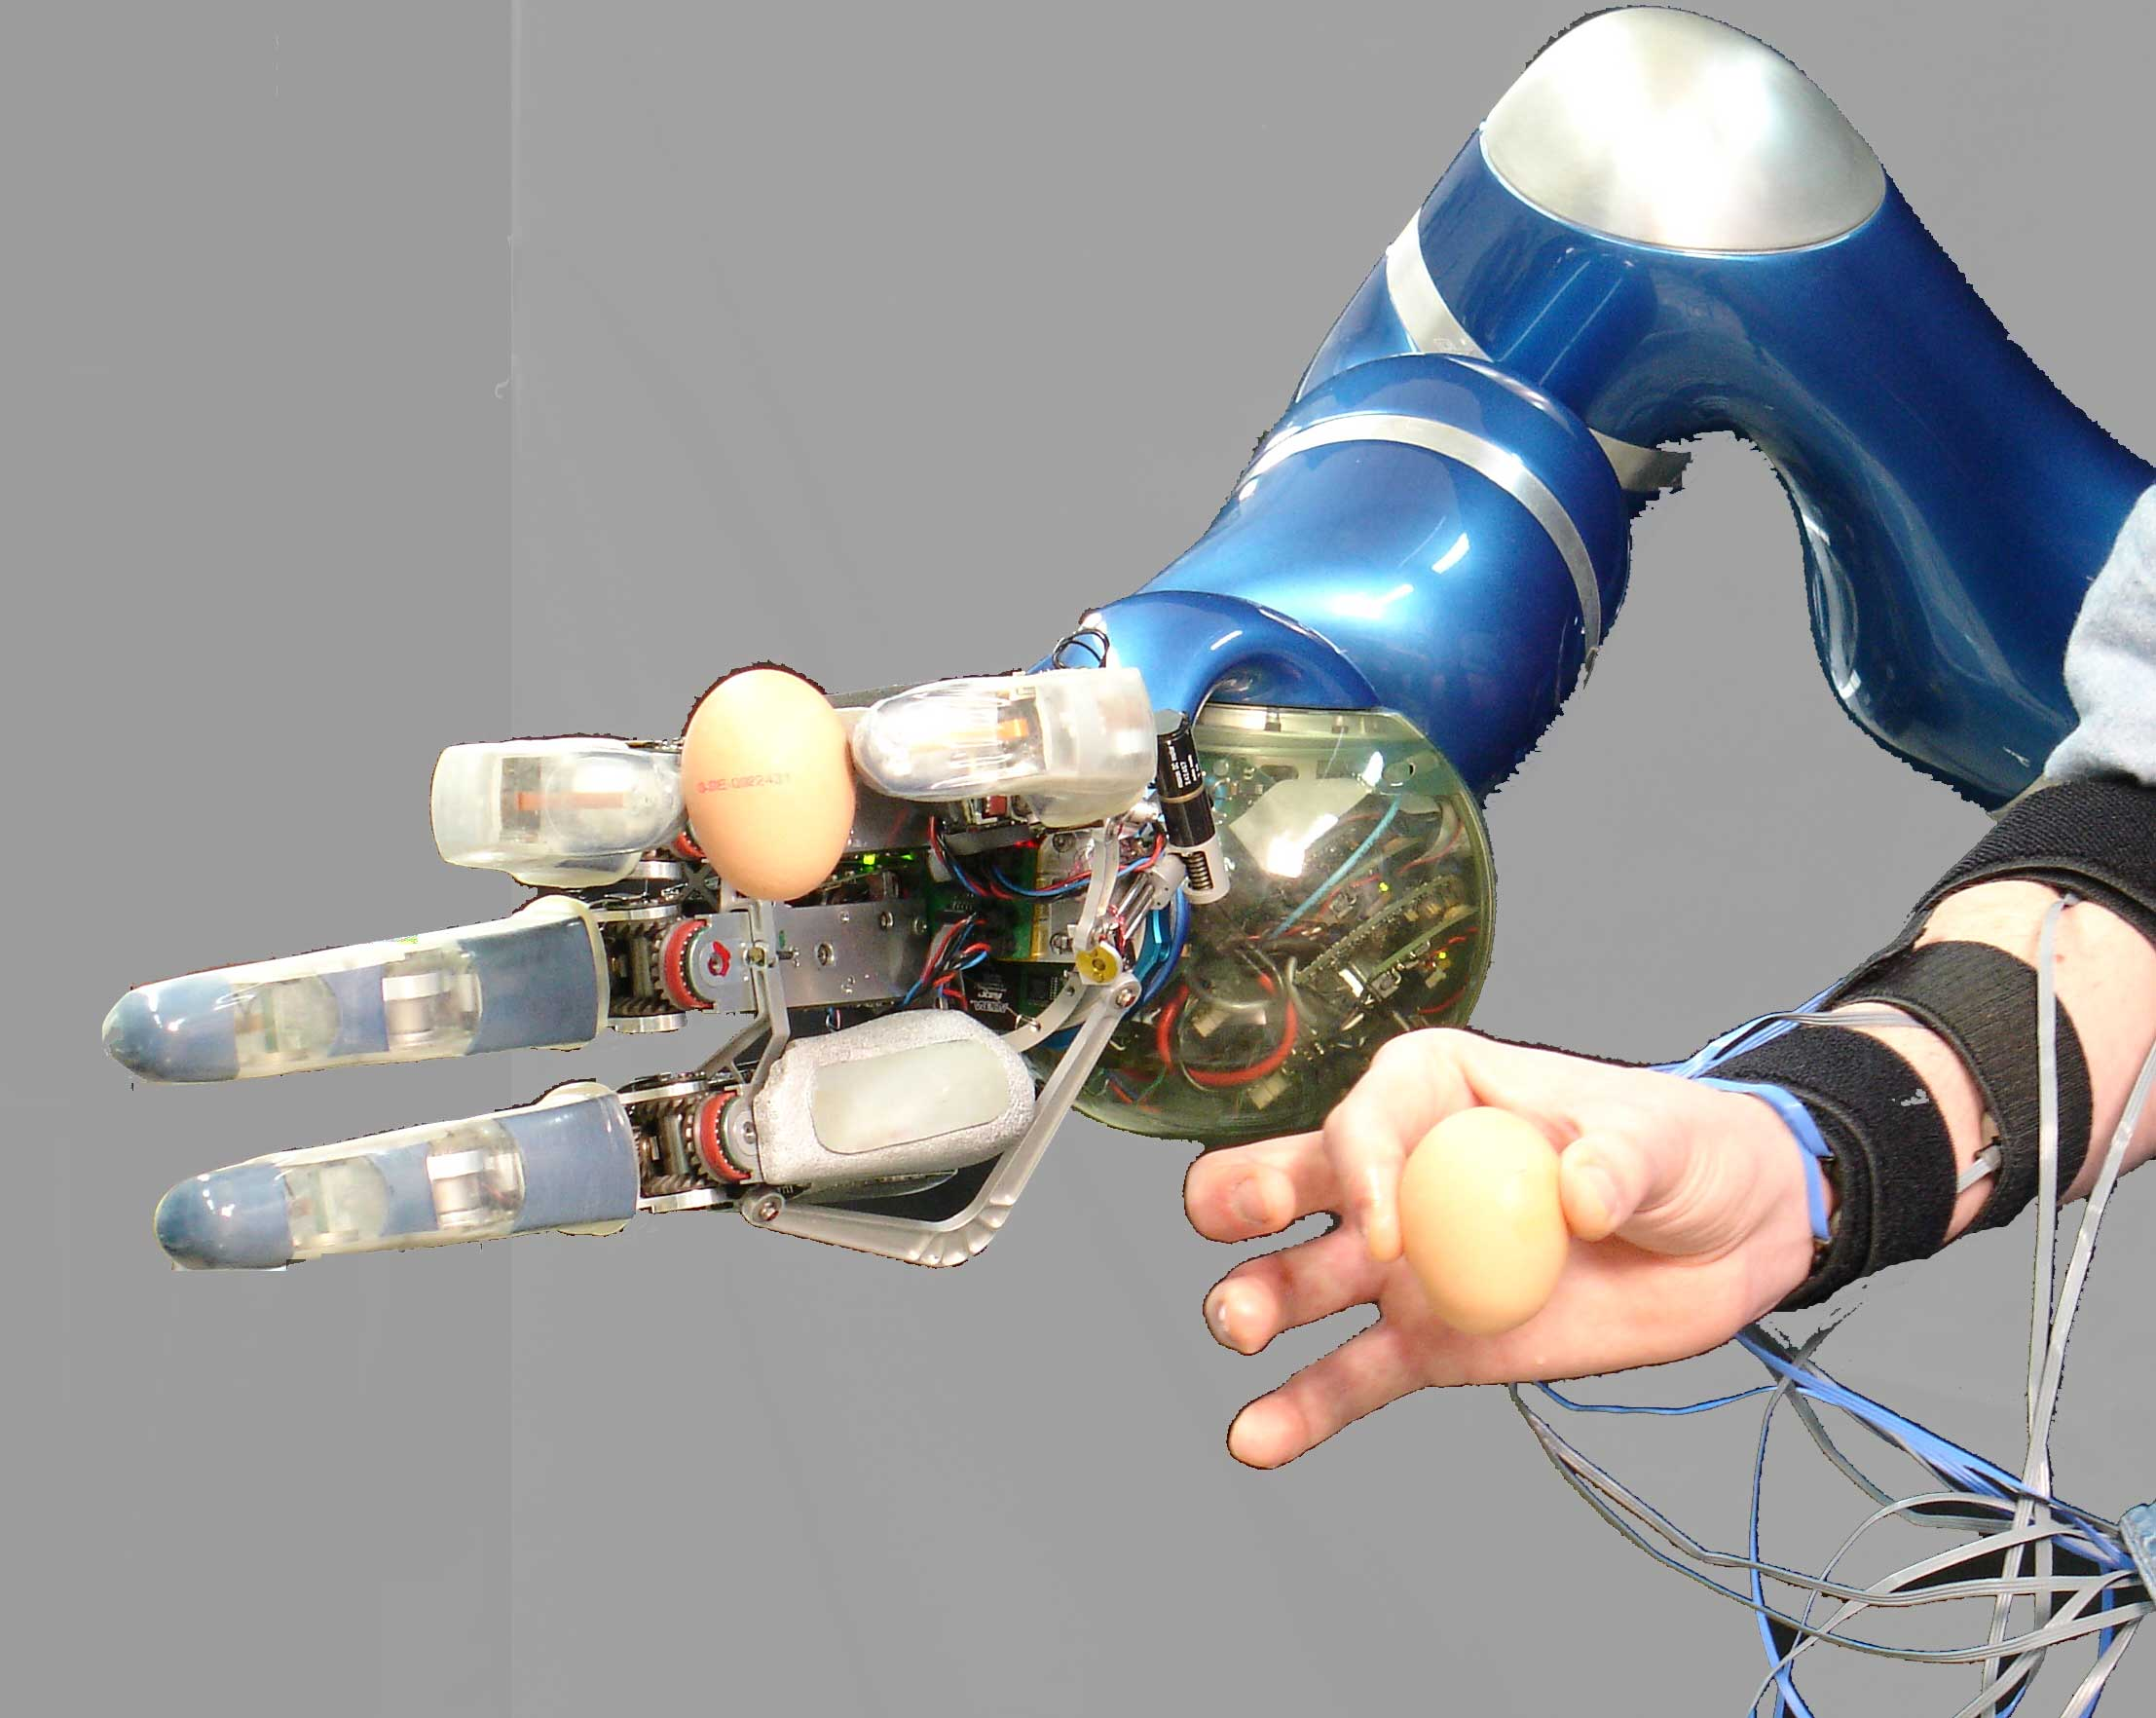
\includegraphics[width=\columnwidth]{figs/egg-in-hand.eps}
  \caption{The DLR four-finger hand II controlled with EMG interface, exerting the right force to hold an egg.}
  \label{fig:egg-hand}
\end{figure}

In the EMG experiment, we used impedance control to exert a force as
generated by the EMG system to hold and grasp object. Example use of
the interface is demonstrated in figure~\ref{fig:egg-hand}. During the
experiment, we verified that the correlation coefficient between the
force applied by the subject and the robot was never less than $80\%$
over a time window of 10 seconds, which let us say that the force
applied by the robot was almost proportional to that applied by the
human subject.
